\question 若平衡二叉树的高度为6,且所有非叶结点的平衡因子均为1,则该平衡二叉树的结点总数为(
~)
\par\twoch{12}{\textcolor{red}{20}}{32}{33}
\begin{solution}解法是一个递推和回归的过程。 递推过程如下: ~ ~ ~ ~

①
高度为6、根结点的平衡因子为1的平衡二叉树由根结点、左子树和右子树组成:~
~ ~ ~

~其左子树应该是高度为5、根结点的平衡因子为1的平衡二叉树。~ ~ ~ ~~

其右子树应该是高度为4、根结点的平衡因子为1的平衡二叉树。 ~ ~ ~ ~

②
高度为5、根结点的平衡因子为1的平衡二叉树由根结点、左子树和右子树组成:~
~ ~ ~~

其左子树应该是高度为4、根结点的平衡因子为1的平衡二叉树。 ~ ~ ~ ~

其右子树应该是高度为3、根结点的平衡因子为1的平衡二叉树。 ~ ~ ~ ~

⑤
高度为2、根结点的平衡因子为1的平衡二叉树由根结点、左叶结点。结点总数为2。
~ ~ ~~

~⑥ 高度为1、即为叶子结点。结点总数为1。~

回归过程: ~ ~ ~ ~设满足条件的高度为h的平衡二叉树中节点总数为ni,有: ~
~ ~ ~n1=1(即为叶结点) ~ ~ ~ ~n2=2 ~ ~ ~ ~n3=n1+n2+1=4 ~ ~ ~
~n4=n3+n2+1=7 ~ ~ ~ ~n5=n4+n3+1=12 ~ ~ ~ ~n6=n5+n4+1=20 ~ ~ ~
~所有本题选B。 【总结】 ~ ~ ~
~平衡二叉树的高度确定,且所有非叶节点的平衡因子确定,平衡二叉树的结构也就确定了。
\end{solution}
\question 若将关键字1,2,3,4,5,6,7依次插入到初始为空的平衡二叉树T中,则T中平衡因子为0的分支结点的个数是(
)
\par\twoch{0}{1}{2}{\textcolor{red}{3}}
\begin{solution}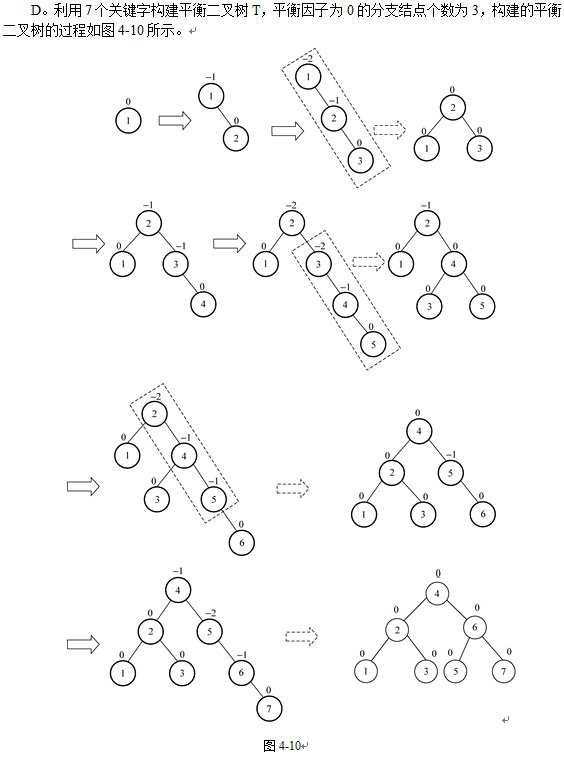
\includegraphics[width=5.87500in,height=7.90625in]{computerassets/36BA3267DBB111192A90D0766834D54C.png}
\end{solution}
\question (中国矿业大学,2004年)AVL树的高度与其节点数N之间的量级关系是( )
\par\twoch{\textcolor{red}{logN}}{}{N}{}
\begin{solution}AVL树的高度对于其节点数N的量级是logN
\end{solution}
\question 输入序列为(20,35,\ldots{}\ldots{}),构造平衡二叉树,当在树中插入值30时发生不平衡则应进行的额平衡旋转是(
)
\par\twoch{LL}{\textcolor{red}{RL}}{LR}{RR}
\begin{solution}平衡二叉树的旋转有4种方式,旋转的过程可以看做以当前节点为根,然后向左旋转或者向右旋转。该题首先将以35为根的树向右旋转,然后将以20为根的树向左旋转,最后得到以30为根的树
\end{solution}
